\documentclass[a4paper, 12pt]{article}
\usepackage[T1]{fontenc}
\usepackage[utf8]{inputenc}
\usepackage[english]{babel}
\usepackage{graphicx}
\usepackage[style=ieee, backend=biber]{biblatex}
%\usepackage[hidelinks]{hyperref}
\usepackage{hyperref}
\addbibresource{bib.bib}
\usepackage{setspace}
\usepackage[nottoc,numbib]{tocbibind}
\usepackage{amsmath}
\numberwithin{equation}{section}

\onehalfspacing

\begin{document}

\title{Flatland Challenge}
\author{G. Berselli, R. De Matteo, M. M. L. Pulici}
\date{July 19, 2021}
\maketitle
\begin{center}
	\fbox{
\includegraphics[width=\textwidth]{Images/Flatland_Logo.jpg}}
\end{center}


\clearpage

\tableofcontents

\clearpage


\section{Introduction}

\subsection{Flatland Challenge}

The aim of the challenge \cite{flatland}, is to achieve efficient management of railway traffic. In particular, this problem is tackled in a simple grid world environment, in order to simulate and experiment different scenarios.

In more detail, the goal consists in making a number of trains arrive at their destinations minimizing the travel time. Even though for simple environments the train can follow explicit plans, as complexity increases the problem of mapping all possible states becomes intractable, for this reason a class of algorithms known as Reinforcement Learning (Section \ref{ch:reinforcement-learning}) can be exploited.

\begin{figure}[h]
	\centering
		\fbox{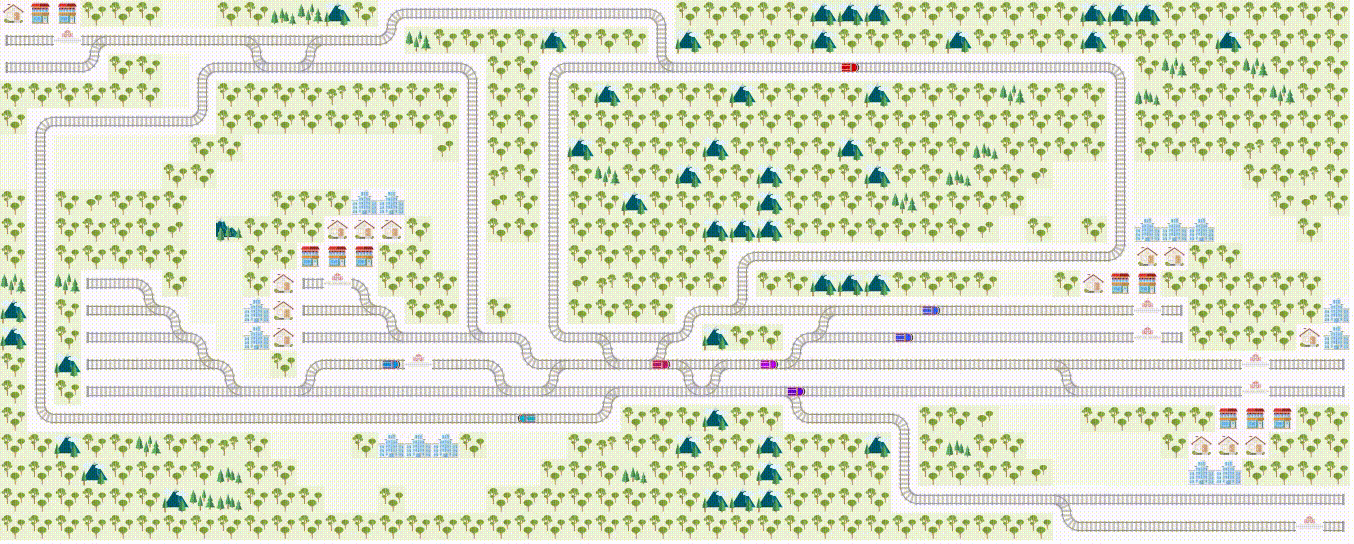
\includegraphics[width=\textwidth]{Images/Flatland_Example.png}}
		\caption{A possible Flatland instance}
\end{figure}

\subsubsection{The environment}

The Flatland environment \cite{flatland-challenge} consists in a discrete time simulation, meaning that each action is performed with a constant time step. At each step, an agent for each simulated train chooses an action. An agent is defined as ``an entity that can move within the grid and must solve tasks'' \cite{flatland-challenge}. More precisely, each agent can choose between two actions: waiting or moving in a direction. Each agent has an individual starting position and its goal is to reach its target destination. Of course, two agents can not occupy the same cell at the same time.

Each cell in the Flatland grid can take the form of any of 8 tile types, as shown in Fig. \ref{fig:cell-types}. More configurations can be obtained by rotating and mirroring the 8 basic tiles.

\begin{figure}[h]
	\centering
		\fbox{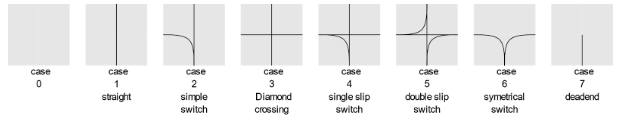
\includegraphics[width=\textwidth]{Images/cell-types.png}}
		\caption{The 8 cell types}
	\label{fig:cell-types}
\end{figure}

When the tile is of the straight type, the agent can only choose to continue moving or to stop. In presence of a simple or a double switch, the train is forced to decide in which of the offered direction to move. When arriving at a dead end, an agent can only stop or go backward.


\subsection{Reinforcement Learning}\label{ch:reinforcement-learning}

The term Reinforcement Learning \cite{reinforcement-learning} refers to the class of agents which rely on feedbacks, or rewards, produced by the agents themselves when interacting with the environment. The way Reinforcement Learning works is to use observed rewards to learn the best possible policy for the given environment. In other words, the agent has no prior knowledge of the environment and must learn how to behave based only on posterior trial-and-error feedbacks.

There are three basic agent designs for Reinforcement Learning:
\begin{itemize}
	\item Utility-based agent, which learns a utility function on states and uses it to select actions;
	\item Q-learning, which learns an action-utility function giving the expected utility of an action given a state;
	\item Reflex agent, which learns a policy mapping directly from states to actions.
\end{itemize}

In addition to these designs, Reinforcement Learning can be either passive, meaning that the policy is fixed and the task is to learn the utilities of states, or active, referring to agents which must also learn how to act.

\subsubsection{Q-learning}

For the Flatland Challenge, Q-learning is used. This class of algorithms learn an action-utility representation instead of simply learning the utilities. The value of an action-state tuple is typically indicated as $Q\left(s,a\right)$. There is a direct correlation between Q-values and state utilities, as expressed by the following equation:
\begin{equation}
	U\left(s\right) = \max_a Q\left(s,a\right).
\end{equation}

The main difference between Q-functions and basic utility information si that no model of the form $P\left(s'|s,a\right)$ is needed, either for learning or for action selection. This characteristic makes Q-learning a model-free method.

At equilibrium, when the Q-values are correct, the following equation must hold:
\begin{equation}
	Q\left(s,a\right)=R\left(s\right)+\gamma\sum_{s'}P\left(s'|s,a\right)\max_{a'}Q\left(s',a'\right).
\end{equation}





















\clearpage
\printbibliography[heading=bibintoc]

\end{document}